\title{CS 613 - Machine Learning}
\author{
        Assignment 4 - Artificial Neural Networks\\
	Alex Lapinski\\
        Fall 2016
}
\date{11/27/2016}
\documentclass[12pt]{article}
\usepackage[margin=0.7in]{geometry}
\usepackage{graphicx}
\usepackage{float}
%\usepackage{comment}
\usepackage{amsmath}
\graphicspath{{./graphs/}}

%\includecomment{versionB}
%\excludecomment{versionB}

\begin{document}
\maketitle

\section{Binary Artificial Neural Networks}\label{Binary ANN}
\begin{table}[h]
\begin{center}
\begin{tabular}{|l|l|}
\hline
Testing Error & 0.337679269883\\
\hline
\end{tabular}
\caption{Binary ANN Testing Error}
\end{center}
\end{table}

\begin{figure}[H]
\begin{center}
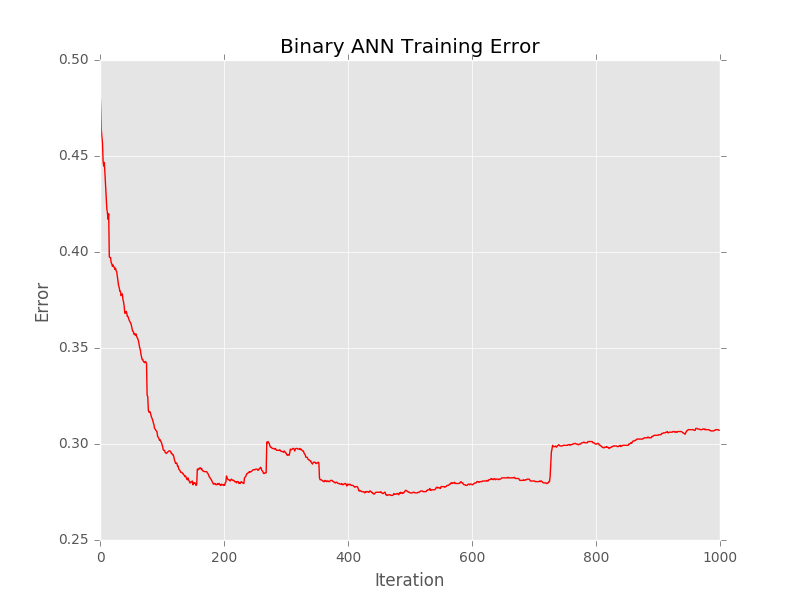
\includegraphics[width=0.9\textwidth]{binary_ann_training_errors.png}
\caption{Training Error for ANN}
\end{center}
\end{figure}

\newpage

\section{The Precision-Recall Tradeoff}\label{Precision-Recall}
\begin{figure}[H]
\begin{center}
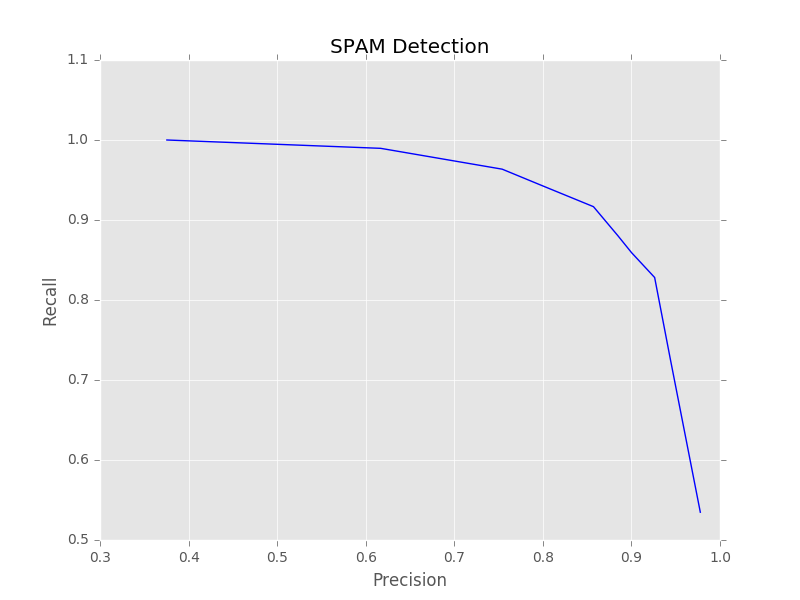
\includegraphics[width=0.9\textwidth]{precision_recall.png}
\caption{PR-Graph for Binary ANN}
\end{center}
\end{figure}

\newpage

\section{Multi-Class Artificial Neural Networks}\label{Multi-Class ANN}
\begin{table}[h]
\begin{center}
\begin{tabular}{|l|l|}
\hline
Testing Error & 0.181946403385\\
\hline
\end{tabular}
\caption{ANN Testing Error}
\end{center}
\end{table}

\begin{figure}[H]
\begin{center}
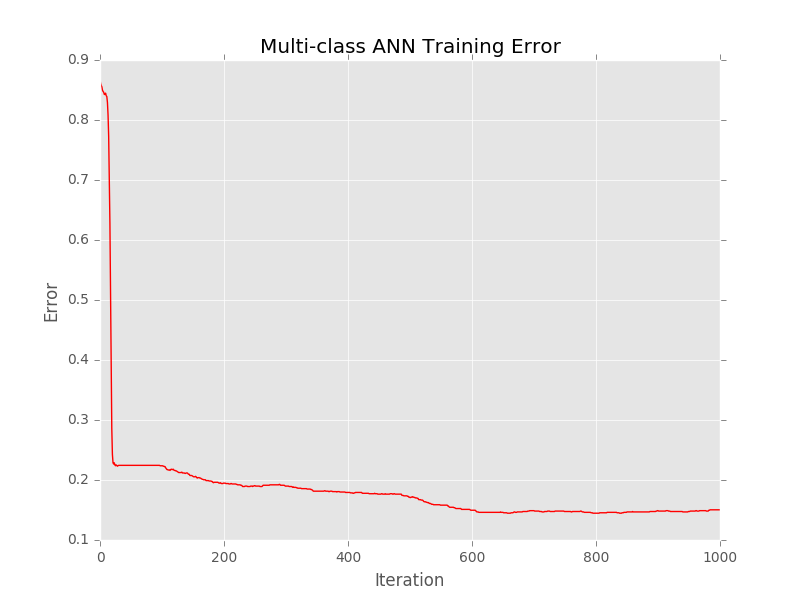
\includegraphics[width=0.9\textwidth]{multiclass_ann_training_errors.png}
\caption{Training Error for Multi-Class ANN}
\end{center}
\end{figure}

\end{document}

